\section{Геометрическая оптика. Принцип Ферма. Законы преломления и отражения. Полное внутреннее отражение.}
\subsection*{Область применения}
\begin{enumerate}
	\item $\lambda \rightarrow 0$, $\frac{\lambda}{D} << 1$
	\item $|\lambda^2 \frac{\partial^2 a}{\partial x^2} << |\lambda \frac{\partial a}{\partial x}| << a$
\end{enumerate}
\subsection*{Законы геометрической оптики}
\begin{enumerate}
	\item Закон прямолинейного распространения света
	\item Закон отражения
	\item Закон преломления
	\item Принцип независимости световых лучей 
	\item Принцип обратимости солнечных лучей
\end{enumerate}
\subsection*{Принцип Ферма}
\begin{enumerate}
	\item Луч света распространяется в пространстве между двумя точками по тому пути, вдоль которого время его прохождения меньше, чем вдоль любого другого пути, соединяещего эти точки.
	\item Свет распространяется между двумя точками по той траектории, оптическая длина которой минимальна.
\end{enumerate}
$$S = \int n(\vec{r}) d l$$
$$E = E_0(r) \exp [i(\Phi(r) - \omega t)]$$
$$k = grad \Phi$$
$$J = \int_{M_0}^{M} k(r)dr = \Phi(M) - \Phi(M_0)$$
Для траектории $L_0$, совпадающей с траекторией луча, векторы $\vec{k}$ и $d\vec{r}$ параллельны, то есть 
$$J = \int_{M_0}^{M} kds = k_0 L_0 (M_0,M)$$
где $L_0$ --- оптическая длина участка $M_0 M$ траектории луча. Если взять какую-либо иную кривую, соединяющую точки $M_0$ и $M$, то вдоль неё векторы $\vec{k}$ и $d\vec{r}$ не параллельны, так что $kds\geq \vec{k}d\vec{r}$. Поэтому вдоль этой кривой окажется 
$$k_0L = k_0 \int_{M_0}^{M} nds = \int_{M_0}^{M} kds \geq \int_{M_0}^{M} \vec{k}d\vec{r} = k_0 L_0 (M_0, M)$$
Откуда следует равенство $L \geq L_0$.
\subsection*{Закон преломления и отражения}
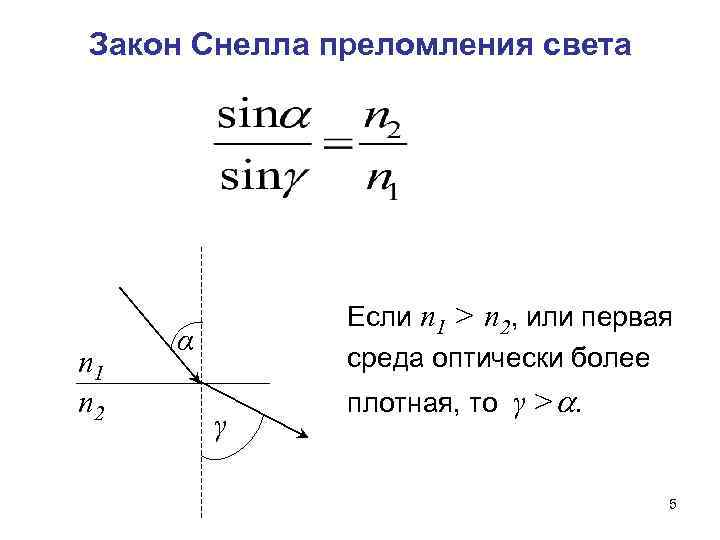
\includegraphics[width=0.5\textwidth]{parts/img/p1_snel.jpg}
$$n_1 \sin \alpha_1 = n_2 \sin \alpha_2$$
$$\alpha_{кр.} = \frac{n_2}{n_1}$$